% === Revtex Declaration ===
\documentclass[]{article}

\usepackage{document_config}
\newcounter{refereecounter}
\newcounter{commentcounter}[refereecounter]
\newcommand{\getcommentlabel}{Comment \textbf{\arabic{refereecounter}.\arabic{commentcounter}}}
\newcommand{\getresponselabel}{Response \textbf{\arabic{refereecounter}.\arabic{commentcounter}}}
\usepackage[margin=0.5in]{geometry}

\newcommand{\ccomment}[1]{
    \vspace{1em}
    \stepcounter{commentcounter}
    \getcommentlabel \\
    \textcolor{darkgray}{\rule{\linewidth}{0.5pt}}
    \color{gray}
    #1
    \color{black}
}
\newcommand{\response}[1]{
    \vspace{1em}
    \getresponselabel \\
    \textcolor{darkgray}{\rule{\linewidth}{0.5pt}}
    #1
}
\setlength{\parindent}{0pt}

\begin{document}
    \begin{center}
        \textbf{Causal Compatibility Inequalities Admitting of Quantum Violations in the Triangle Structure} \\
        \textbf{[Referee Responses]} \\
        Thomas C. Fraser and Elie Wolfe \\
        Perimeter Institute for Theoretical Physics, Waterloo, Ontario, Canada, N2L 2Y5 \\
        University of Waterloo, Waterloo, Ontario, Canada, N2L 3G1\\
        June 7, 2018
    \end{center}

    To begin, we would like to thank both referees for their insightful comments and constructive criticisms. Evidently, the referees understood the subject matter and were diligent in crafting their helpful comments. Therefore, we must sincerely thank the referees for their time and appreciate their expertise. Below we have responded individually, where applicable, to the referees' comments. Our responses are in black text, and the referees' original comments are in gray text. Overall, there were zero comments we disagreed with and we believe that each comment has directly or indirectly led to an improvement of our original submission.

    \stepcounter{refereecounter}
    \section{Responses to First Referee}

    \ccomment{This work considers the derivation of tests for discriminating classical correlations from non-classical correlations in a three-party scenario in which causal influences are pairwise shared between all three players. Hence it is a "triangle scenario". The authors apply the recently developed inflation technique to derive several new inequalities satisfied by all classical correlations in the triangle scenario. Next, they numerically study the ability of quantum theory to violate them. A quantum distribution that doesn't have a classical model has previously known -- Fritz's distribution. This distribution has a central role for how the authors approach the problem. In particular they manage to derive inequalities, robust to a small amount of noise, that detect Fritz's distribution, and some `similar' quantum distributions.}

    \ccomment{This is a long and quite technical paper. Having read it, I understand that it is directed at a specialist audience knowledgeable on causal inference and/or network Bell inequalities. The comments that follow are made with this specialized audience in mind.}

    \ccomment{As the original work, presented in sections VI to VIII, is heavy based on numeric and the computer-implemented inflation technique, I have not considered it reasonable to try to check the correctness of any derivations or numerical claims. I simply trust the authors on this matter.}

    \ccomment{I think the paper is well-written. I had no troubles understanding the messages the authors presumably wished to convey. However, the paper is quite long. Therefore, I think it would benefit from a short and clear summary of what the main contribution of this paper is, and what the outlook is. This appears currently in the conclusions. However, I think it is worth outlining this much earlier in the paper, so that a reader knows what to expect from the long read. Practically, I am proposing that the part of the introduction in which the structure of the paper is presented, is expanded or supplemented.}

    \response{
        Fantastic suggestion; we have updated and adjusted the introduction to make the contributions of this paper more clear to the reader in two ways. First, when summarizing the organization of the manuscript, we make it explicit that the first half is dedicated to a review of previous works, while the second half includes the contributions made by the research. Second, when delineating the precise contributions made by the second half of the paper, we provide an overview of the main purposes for deriving these inequalities and how we explored their utility. The language used now more closely mirrors that of the conclusions. Hopefully, readers familiar with at least the subject matter of Bell inequalities will be able to comprehend the nature of the advancements made by this work from the introduction alone.
    }

    \ccomment{In general I appreciate this type of thorough basic research on a poorly understood topic by, due to currently lack of deep understanding, non-rigorous methods. I think it provides useful hints and shows the potential usefulness of the inflation technique for future work in this direction. By now, I believe it is well-established that it is a difficult matter to study quantum correlations in the triangle scenario. Therefore consider this type of investigations relevant.}

    \ccomment{I consider this paper suitable for PRA, since many previous works on quantum networks have been published here and therefore the right audience will probably notice it. I recommend it for publication, given that my more detailed comments, appearing below, are taken into consideration before either being (partially) addressed or discarded with a good motivation.}

    \ccomment{Regarding section VI. What is previously known about the inequalities of [21] and and [19]? Has nobody studied or attempted to violate these before? If yes, what were the results? I would be a bit surprised if triangle inequalities were derived but attempted to be violated by some super-classical model. Basically, I think it would be good to put the numerics for these inequalities into a bit more of a context.}

    \response{
    We thank the referee for this excellent comment. We have elected to add more historical context to Section VI. Specifically, the first paragraph now reads,

    ``As a preliminary search for quantum incompatibility in the Triangle structure, we performed numerical optimizations (in search of violation) against the previously-published compatibility inequalities of Wolfe et al. [21], as well as against the entropic inequalities of Henson et al. [19]. For historical context, the entropic inequalities of [19] have already been independently investigated for quantum incompatibility by Weilenmann and Colbeck [20] using a variety of computational methods. Unfortunately, these methods failed to identify quantum-accessible distributions capable of violating any of the entropic inequalities considered by [20]. Additionally, the inequalities presented in [21] have not been previously investigated numerically.''

    For even more context (excluded from Section VI for brevity), entropic inequality constraints for the Triangle structure first appeared in Fritz, Chaves [40], but a completed list of all Shannon-type entropic inequalities was not computed in [40] due to the computational limitations of the Fourier Motzkin elimination procedure. In Chaves, Luft, and Gross [17], these computational limitations were overcame using all conditional independence constraints present in the Triangle structure to pre-process the Fourier Motzkin procedure and produced two new entropic inequalities. To the best of our knowledge, attempts to violate these inequalities using computational methods first appeared in [20].
    }

    \ccomment{In addition, I am a bit puzzled by the following comment "These early results suggest that there is no quantum-classical gap in the Triangle structure for two-outcome measurements". Although I am personally prepared to believe this for various reasons, I do not see how the numerical study of the particular inequalities of [21] and [19] justifies it?}

    \response{
    The referee is correct. Strictly speaking, the numerical failings are inconclusive. The purpose of the `conjecture' was to narratively motivate the shift to larger-outcome inequalities. The document now reflects a more conservative perspective:

    ``Unfortunately, these early results are inconclusive for two reasons. First, an exhaustive search would need to consider the possibility of larger Hilbert spaces for the shared quantum states. Second, there is little reason to suggest that the inequalities considered in [21] are complete; it is possible there are other constraints on two outcome distributions for the Triangle structure yet to be discovered.

    Nonetheless, having failed to observe a quantum-classical gap in the Triangle structure for \textit{binary-outcome} measurements, a continued search for \emph{non}-classical distributions in the Triangle structure must expand the gamut of inequalities to optimize against to include inequalities referencing strictly more than two outcomes.''
    }

    \ccomment{ Disregarding that (what I understand is) optimization from the interior of the quantum set, cannot prove the correctness (indeed only “suggest” the correctness) of such a statement, one would still need to know a thing or two about the properties of the inequalities considered. For example, the classical set is non-convex so there is no notion of a facet. Are the inequalities in [21] and [19] `optimal', so that the inability to violate them somehow indicates the lack of a quantum advantage for any inequality? If yes, what would it mean that an inequality in a non-convex setting is optimal? Furthermore, is it uniquely optimal, or can there be other unknown optimal inequalities where we could find a quantum violation? In summary, I wonder whether the claim is properly motivated.}

    \response{
        Excellent question. Evidently, the notion of a facet breaks down when the set of classical correlations no longer forms a polytope. The Triangle structure is an instance of this breakdown. Geometrically, an inequality is considered `tight' if its intersection with the classical/compatible set is full-dimensional (i.e. the surface of intersection has dimension one less than the embedding dimension).

        More formally, new results due to Rosset, Gisin, Wolfe (\url{https://arxiv.org/abs/1709.00707}) reveal that it is possible to generalize the notion of an 'optimal' inequality. Explicitly, in 1709.00707, it was proven that the set of compatible classical distributions for any causal network (including the Triangle structure) forms a semi-algebraic set; meaning that there exists a \textit{finite} list of inequality and equality constraints that are necessary and sufficient for accessing compatibility. Therefore, an inequality belonging to this necessary and sufficient set may be considered as optimal.

        Determining whether or not any given inequality is optimal in this sense is still poorly understood and certainly worthy or further research. For the sake of brevity, we elected to include the following sentence to Section VI.

        ``Second, there is little reason to suggest that the inequalities considered in [21] are complete; it is possible there are other constraints on two outcome distributions for the Triangle structure yet to be discovered.''
    }

    \ccomment{Regarding the new inequalities. Do the authors have some intuition for what type of inflations leads to interesting inequalities? It is stated that larger inflations were needed, as compared to those of ref [21]. Is it the case that the larger the inflation, the stronger the inequality? Furthermore, as far as I understand, a given inflations leads to many possible inequalities. Is there natural way to identify the interesting inequalities, or must check them one by one to find the interesting results? Again, if the authors have developed further intuition for such practically relevant matters of how to best use inflation, it would be good to mention it in the main text.}

    \response{
        Excellent questions. Your intuition is correct, larger inflations lead to stronger inequalities. This is proven in [22] by demonstrating that the Inflation Technique is capable of completely solving the causal compatibility problem. Explicitly, if a distribution is incompatible with a causal structure, then there exists a sufficiently large inflation capable of generating an inequality which witnesses its incompatibility. Nonetheless, the inequalities derived in the paper came from relatively small inflations. Our revision of the paper now expands on this point,

        ``The Inflation Technique is known to completely solve the causal compatibility problem through increasing orders of inflations [22]. Consequently, the derivation of Ineqs. (13,15,12) is guaranteed by [22] for sufficiently large inflations. Nonetheless, the following inequalities were obtained using the relatively small inflations found in Fig. 8.''

        In a footnote,
        ``Note that the adjectives large and small used to describe an inflation only become well-defined in the context of the hierarchy proposed in [22]. For example, the Web Inflation in Fig. 8c is second in the hierarchy of [22] whereas the Wagon-Wheel Inflation in Fig. 8b is somewhere between the first and second order.''

        Regarding the generation of many possible inequalities, the referee is correct. In the absence of a particular distribution, the Inflation Technique yields a plethora of inequalities, many of which are redundant (strictly speaking, this problematic feature is shared among many inequality-deriving techniques which use linear (or non-linear) quantifier elimination). If the objective is to identify which of the non-redundant inequalities admit quantum violations, the best method (for the moment) is to check them one by one. However, in this paper we used a method (explained in Appendix C) for deriving inequalities in the presence of a particular distribution, namely the Fritz distribution. This method only produces inequalities which by construction are violated by the Fritz distribution already; therefore we avoid having to distinguish the interesting inequalities from the uninteresting ones. As such, the task of eliminating uninteresting inequalities never naturally arises in this paper. Moreover, the original Inflation paper [21] addresses most of these concerns and comments in a more universal setting (i.e. for any causal structure, not just the Triangle structure), and consequently, we have found it best to omit the topic from this paper.
    }

    \ccomment{Regarding genuine quantum triangle correlations. I fully agree with the authors that the Fritz distribution is manufactured to fit the triangle scenario based on the well-known CHSH violations. Indeed, this is not a genuine triangle correlation. This is sufficient to convince a reader that not all quantum violations of a triangle inequality are qualitatively interesting. However, an important issue would be to define what it means that a quantum triangle correlation is not based on Bell's theorem. The authors inherit this question from the work of Fritz. Although agreeing with the intuition, I think the intuition for this question is not yet sufficiently developed to be phrased as a meaningful question. Basically, what does it mean for a general probability distribution in the triangle not to be based on Bell's theorem?}

    \response{
        See our response to \textbf{1.14}.
    }

    \ccomment{The authors have derived a triangle inequality with a quantum violation that is not identical to the Fritz distribution. Nevertheless, they make the following comment (in the conclusions):}

    \ccomment{"Despite these advancements, the distributions we discovered hew closely to the Fritz distribution, indicating that their non-classical nature remains some recycled version of the non-classicality found in the Bell structure. Currently, it remains speculative about how to recognize whether-or-not a given distribution for the Triangle structure exhibits non-classical correlations of a fundamentally novel qualitative nature than Bell-type non-classicality."}

    \ccomment{The inability to address my above question (what does it mean for triangle correlations not to be based on Bell's theorem?) hinders the authors to make a clear conclusion about their not-identical-but-quite-similar-to-Fritz's distribution. I would consider this an important question since it is essential to how strong a conclusion can be drawn from one of the key result of the paper. I am mildly surprised that the authors did not make an effort to at least partially address this matter. Perhaps the question could (at least) be rigorously formulated, i.e., a reasonable definition could be provided for what it means for triangle correlations not to be based on Bell's theorem. However, without knowing how such a definition may look, I suspect that resolving the question will not be straightforward. Nevertheless, it may be worth it for the authors to draw some attention to this poorly defined but clearly relevant idea.}

    \response{
        This comment \textbf{1.14} and the above comment \textbf{1.11} will be answered here.

        Determining whether or not a given quantum correlation incompatible with the Triangle structure expresses genuine, novel forms of non-classicality is, at the moment, not yet a sufficiently developed decision problem as the referee mentions. Moreover, we completely agree that is worth drawing attention to this clearly relevant idea. As such, we have included in the resubmission a new section that precedes the conclusion titled Revisiting Fritz's Problem. In this section, we consider a few avenues for formalizing this idea, and point out a deficiency for each. Ultimately, this additional section fails to rigorously reformulate Fritz's problem, but at least provides the reader with an understanding for the importance of doing so.
    }

    \clearpage
    \stepcounter{refereecounter}
    \section{Responses to Second Referee}

    \ccomment{This paper reports on the use of the inflation technique to derive inequalities for the triangle causal structure that admit quantum violations. The triangle causal structure is a well-studied example and seems to be resistant to being solved elegantly. The authors make progress on this difficult problem, while still not getting to an elegant solution. However, the progress they make is interesting and qualitatively different to before, since the inequalities found are the first that are known to have quantum violations (there are many existing inequalities not known to have such violations).}

    \ccomment{I am happy to recommend this be accepted subject to minor changes.}{}

    \ccomment{
    More detailed remarks/comments/questions:

    Introduction:

    It is perhaps a bit strong to claim that *every* aspect of quantum phenomena that is non classical had led to practical exploitation for computation or communication. [note the typo "of"-\textgreater"or" shortly before [4]]
    }

    \response{Agreed. Typo corrected. Modified sentence: ``Throughout history, numerous quantum phenomena which fail to be emulated by classical physics have been identified as resources for solving computational or communicational problems.''}

    \ccomment{Sentence "This work is the first therefore...", should perhaps say "known" rather than "able"}

    \response{Corrected.}

    \ccomment{Related to the same paragraph, isn't is implied by [22] that such inequalities must exist in principle? Is one conclusion of the present paper that one doesn't have to go too far down the inflation chain to find one?}

    \response{
        Correct, [22] proves that some inequality will be found at some sufficiently high order in the inflation hierarchy. The inflations consider in this paper are all relatively low on the hierarchy. However, when one expects to find an inequality (if there is one) is still poorly understood. For example, in [28] there is a $4$-outcome distribution for the Triangle structure which is conjectured to be incompatible and yet it passes the second order inflation tests failed by the Fritz distribution. The following addition is made to Section V II:

        ``The Inflation Technique is known to completely solve the causal compatibility problem through increasing orders of inflations [22]. Consequently, the derivation of Ineqs. (13,15,12) is guaranteed by [22] for sufficiently large inflations. Nonetheless, the following inequalities were obtained using the relatively small inflations found in Fig. 8. This efficiency is not universally guaranteed; for comparison, we remark that unlike the Fritz distribution, the conjectured incompatibility of the 4-outcome distribution proposed by [28] is not confirmed by Inflation Technique at the same level.''

        See also response \textbf{1.10}.
    }

    \ccomment{
    Sec II:

    Sentence "Specifically, the causal structure G hypothesizes..." has grammatical issues.}

    \response{Agreed. Modified sentence: ``A causal structure $\graph$ hypothesizes that each variable $n \in \nodes$ is only directly influenced by its parents $\Pa[\graph]{n}$.''.}

    \ccomment{Near the end of Sec II, "complete characterization for any causal structure": this remark clashed with a later remark on p5 that Bell's structure has a "complete classification of classicality".}

    \response{Corrected: Currently however, it is unknown how to obtain a complete characterization for all causal structures, including the Triangle structure.}

    \ccomment{
    Sec III:

    typo "asses"-\textgreater"assess"}

    \response{Corrected.}

    \ccomment{In (2) there is a P\_lambda missing after the sum.}

    \response{This is a typo in the ArXiv submission and was corrected for our PRA submission.}

    \ccomment{
    Sec V:

    Perhaps change "We close this loophole..." to "This loophole is closed..." to make clear this is not a new idea here.}

    \response{Corrected: ``This loophole is closed by having...''.}

    \ccomment{
    Sec VII A:

    Last paragraph, maybe write P\_ABC as P\_\{A\_lA\_rB\_lB\_rC\_lC\_r\} or mention equivalence: if I understand correctly, the alphabet size must be 4 for each of A, B and C to use (11).}

    \response{
        Apologies for the confusion, this equivalence has now been explicitly mentioned. Moreover, we believe that the ordering of statements in Section V made it very confusing for any reader to understand the two different, but isomorphic notations. As such, we have made slight modifications to Section V to make this correspondence clear for future readers.
    }

    \ccomment{typo "distribution very similar to P\_F itself" -\textgreater "distributions"}

    \response{Corrected.}

    \ccomment{Do you have any insights as to why the particular inflations considered turn out to be useful? Do you have any insight as to which inflations are likely to be useful?}

    \response{
        Initially, the particular inflations considered were chosen with the intuition that ``larger'' inflations might be capable of generating new inequalities. Moreover, inflations ``larger'' than the Web inflation became computationally demanding for investigations. Overtime, more intuitions and insight began to develop. For example, the Wagon-Wheel inflation is not an arbitrary choice. In the Bell structure, both Alice $A$ and Bob $B$ have two settings. Therefore, in order to capture this idea in an inflation of the triangle structure, we needed to construct two copies of Alice $A_1$, $A_2$, and Bob $B_1$, $B_2$, and consequently two copies of settings variables $X_{1}, X_{2}$ and $Y_{1}, Y_{2}$. As pointed out in Section V, the role of Charlie $C$ is to document and announce all distinct pairs of settings and therefore at least four $C$'s are ``needed''. These observations suggest the Wagon-Wheel inflation is worth considering. In this sense, we might have expected the Wagon-Wheel inflation to be useful. At the moment, we have yet to develop a systematic and universal understanding of these vague intuitions and insights. Therefore, we elected to omit these imprecise discussions from the paper and have differed these ideas for future research.

        See also response \textbf{2.5}.
    }

    \ccomment{I'm not sure the figures of distributions are presented in the best way: given that (if I understand correctly) there are only 3 different values in Fig 5, for example, why not just state these individually (like is done for the white value) rather than give the scale of values.}

    \response{ Great point. Figures 4 and 5 have been tweaked to simply state the three probability values. }

    \ccomment{
    Sec VIII:

    "..initial parameters such that the initial point of the optimization was close to P\_F.": can you say more about what "close" means? Were all parameters varied or only the nonzero parameters?}

    \response{
        Here ``close'' means close with respect to a Euclidean norm in parameter space. These nearby points in parameter space were obtained by first constructing parameters which reproduce $P_{F}$ exactly. Then for each individual parameter $\lambda$ in this set, we sampled a perturbation $\de \lambda$ from a Gaussian distribution with standard deviation $\sigma = 2\pi 10^{\chi}$. Then we seeded the numerical optimization with $\lambda + \de \lambda$. If we let $\chi$ become too large (approximately $\chi > -1.5$), the numerical optimization would converge to parameters that generate saturating distributions. For $\chi$ sufficiently small, the optimization would converge to parameters that generate violating distributions. In this sense, all of the parameters were varied, not just the non-zero parameters. Below is a plot (left), and the same plot zoomed in (right), illustrating this phenomena.
        \begin{center}
            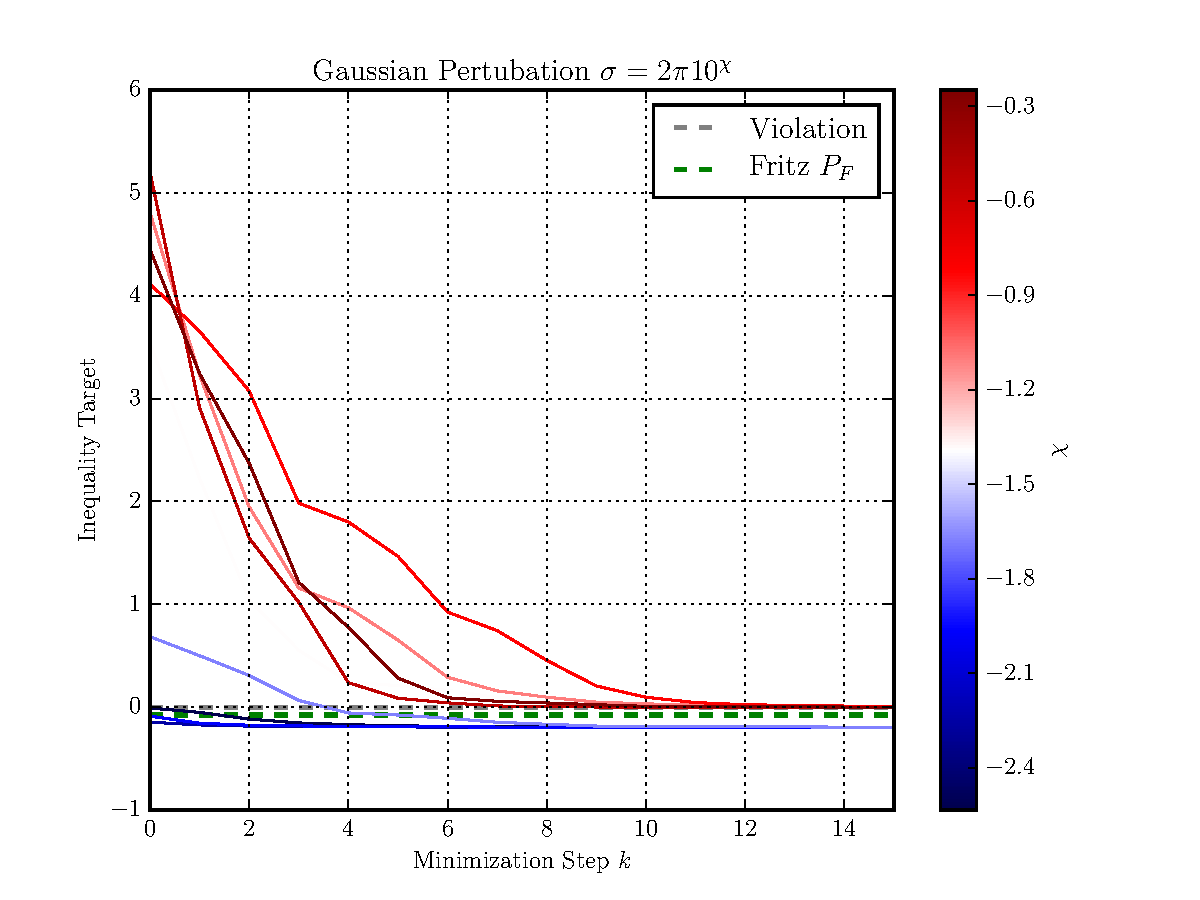
\includegraphics[scale=0.4]{Gaussian_Perturbation_Fritz_Color_Default.pdf}
            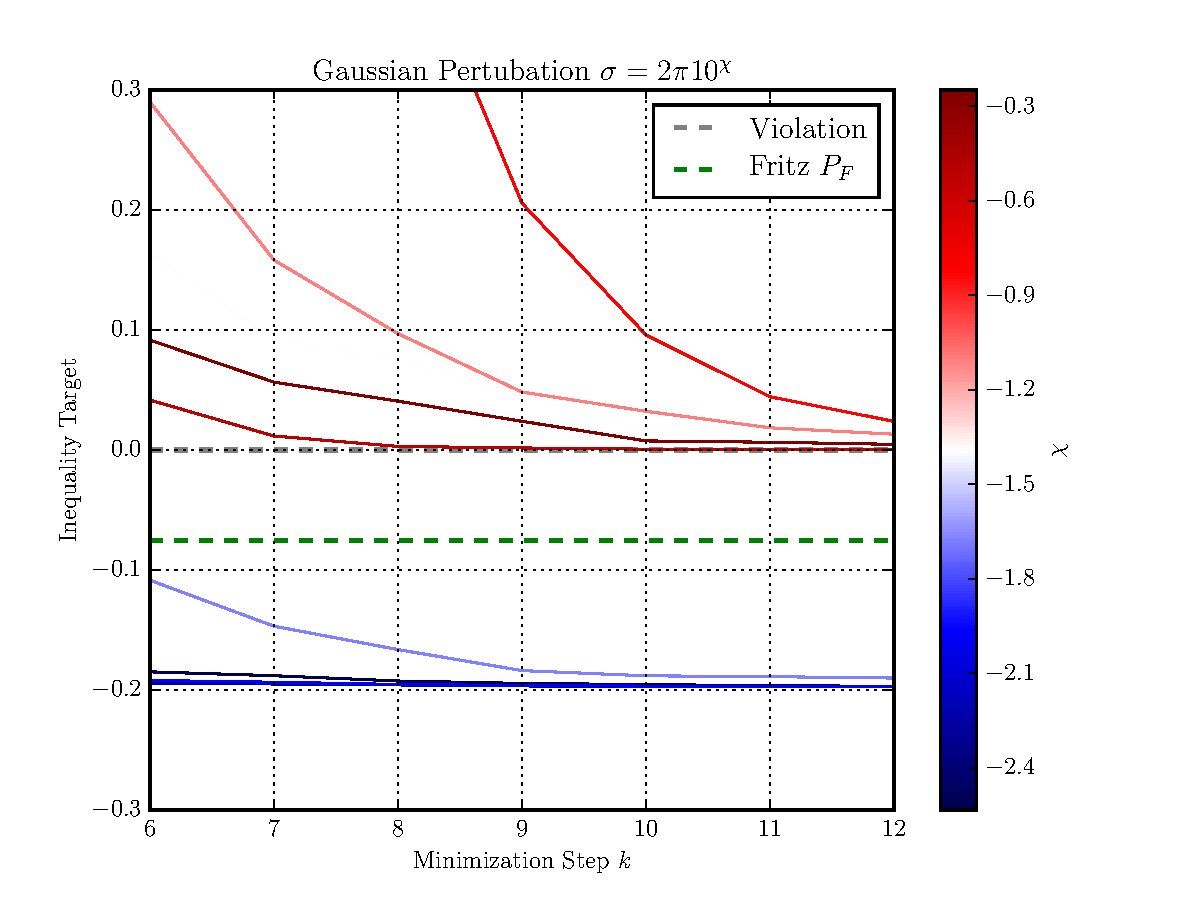
\includegraphics[scale=0.4]{Gaussian_Perturbation_Fritz_Color_Zoomed.pdf}
        \end{center}
    }

    \ccomment{"...violating it suboptimally than P\_F.": reword}

    \response{Reworded sentence: ``To the contrary, our numerical optimization failed to find any symmetric quantum distributions capable of violating $I_{\text{SymmetricWeb}}$''.}

    \ccomment{
    Conclusions:

    Perhaps it is misleading to say that no noise is tolerated by Fritz's argument: his argument works for noisy entangled states (provided CHSH is still violated). Perhaps it is less obvious what happens when noise occurs elsewhere, but the other parts need only classical resources to realize in which case noise is less problematic. I would also imagine that even if it not literally robust as written that it could be made robust fairly easily.}

    \response{
        The referee is correct in saying that if the entangled quantum state shared between $A$ and $B$ is subjected to noise, then provided that CHSH is still violated, Fritz's argument still holds. Crucially however, the argument requires \textit{perfect} correlation between $C$ and the left bits of $A$ and $B$. Therefore, introducing \textit{any} amount of noise to the classical resources which establish these perfect correlations prohibits one from applying Fritz's argument with absolute confidence. Nonetheless, we \textit{are} sympathetic to sharing the referees intuition as a means of a priori expecting that \textit{some} amount of noise is tolerable, but the important question is how much noise? The robustification of Fritz’s argument is precisely what this paper accomplishes using the Inflation Technique. It is our hope that further research will identify a more direct/simple route for performing these robustifications in general.
    }

    \ccomment{grammar: "a causal compatibility inequalities"}

    \response{Corrected: ``...it was demonstrated that these causal compatibility inequalities are robust to noise...''.}

    \ccomment{"advantages from a resource perspective": it isn't clear to me what you are referring to, so please add some explanation or reword.}

    \response{
        Apologies for this confusion. An earlier draft had a more detailed explanation of what we mean by a ``resource perspective'' but was subsequently omitted before our original submission. We have decided to remove this comment from the conclusion entirely. Remnants of these ideas have been re-introduced in the new section titled Revisiting Fritz’s Problem (see Response \textbf{1.14}).

        Specifically, the original idea was as follows. In order to find new examples of novel quantum resource in the Triangle structure, perhaps one might need to require the three parties $A,B,C$ to perform some correlation game/task using the latent resources of the Triangle structure. In particular, one could ask what correlations are achievable using only a single quantum state, or two quantum states, or all three. Since Fritz distribution can be achieved with only a single quantum state, maybe distributions which need to exploit the quantum resources of all three exhibit a type of non-classicality distinct from the Fritz distribution.
    }

    \ccomment{p14 typo: "which be solved"}

    \response{Corrected: ``...which can be solved efficiently...''.}


    % \nocite{apsrev41Control}
    % \bibliography{references}

\end{document}